
\setcounter{page}{26}
\setlength{\columnsep}{26pt} % расстояние между колонками

    \begin{multicols}{2} % начинаем две колонки 
    \vspace*{0.2mm} % отступ в начале для первой колонки
    \section*{Решения задач} % заголовок   
    \small\textbf{M170---M173; Ф188---Ф192} % подзаголовок

    \vspace{35mm} % отступ между заголовком и основным текстом
    
    \noindent\textbf{M170.} 
    \textit{a) Пусть $M$ и $N$ - точки касания окружности, вписанной в треугольник $ABC$, со сторонами $AB$ и $AC$, $P$ - точка пересечения прямой $MN$ с биссектрисой угла $B$. Докажите, что угол $BPC$ прямой.}\par
    
    \textit{б) Докажите более общий факт: если точка O, расположенная внутри треугольника, такова, что $\measuredangle BOC$ --- $\measuredangle BAO = 90^\circ$, $M$ и $N$ --- основания перпендикуляров, опущенных из точки $O$ на стороны $AB$ и $AC$, $P$ --- точка пересечения прямых $BO$ и $MN$, то $\measuredangle BPC = 90^\circ$ (рис. 1).}\par
    
    \vspace{2mm}
    
    Задача а), действительно, частный случай б): если $O$ --- центр вписанной окружности, то $BOC$ в сумме с углами $OCB$ и $OBC$ равен $180^\circ$, а $\measuredangle BAO$ в сумме с теми же углами равен половине суммы углов треугольника, то есть $90^\circ$.\par Поэтому решим сразу задачу б). Пусть
    для определенности точка $P$ лежит на про-
    должении отрезка $MN$ за точку $N$, как на нашем рисунке. (Другие случаи разбираются аналогично, вы без труда справитесь с ними самостоятельно.) По условию $\measuredangle OMA = \measuredangle ONA = 90^\circ$, поэтому вокруг четырехугольника $OMNA$ можно описать окружность, следовательно,
    $$\measuredangle ONM = \measuredangle OAM = \measuredangle BAO.$$
    Покажем теперь, что точки $O$, $N$, $P$ и $C$ ле-
    
    \vspace{2mm} % расстояние между треугольником и текстом
    
    \begin{center}
        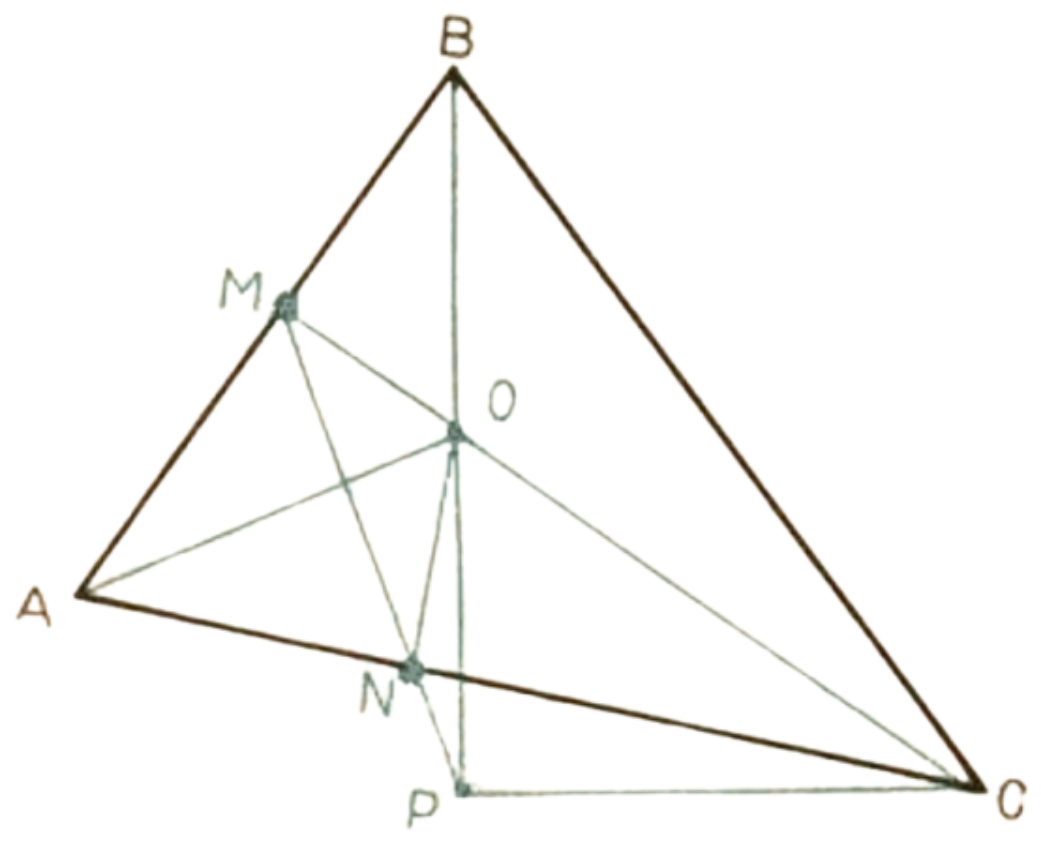
\includegraphics[width=0.849\columnwidth]{triangle.png}
        \captionof{figure}{}
    \end{center}
   
    \columnbreak
    
    \noindent жат на одной окружности. Действительно,\par
    $\measuredangle CNP = \measuredangle MNA = 90^\circ - \measuredangle MNO = 90^\circ - \measuredangle BAO, \measuredangle COP = 180^\circ - \measuredangle BOC.$\par\noindent Используя условие задачи: $\measuredangle BOC - \measuredangle BAO = 90^\circ$ получаем \par {\centering $\measuredangle CNP = \measuredangle COP$.\par} \noindent Наконец, из того, что четырёхугольник $CONP$ вписанный, следует нужное нам равенство \par {\centering $\measuredangle CPO = \measuredangle CNO = 90^\circ$.\par} \hfill \textit{И.Ф.Шарыгин}
    \vspace{1mm}

    {\noindent\textbf{M171.}} \textit{На плоскости нарисован правильный шестиугольник, длина стороны которого равна 1. При помощи только линейки построить отрезок длины $\sqrt7$}.\par Вы без труда докажете, что длина красных отрезков на рисунке 2 равна $\sqrt7$.
    %\vspace{1mm} % отступ между шестиугольниками и текстом
    \begin{center}
        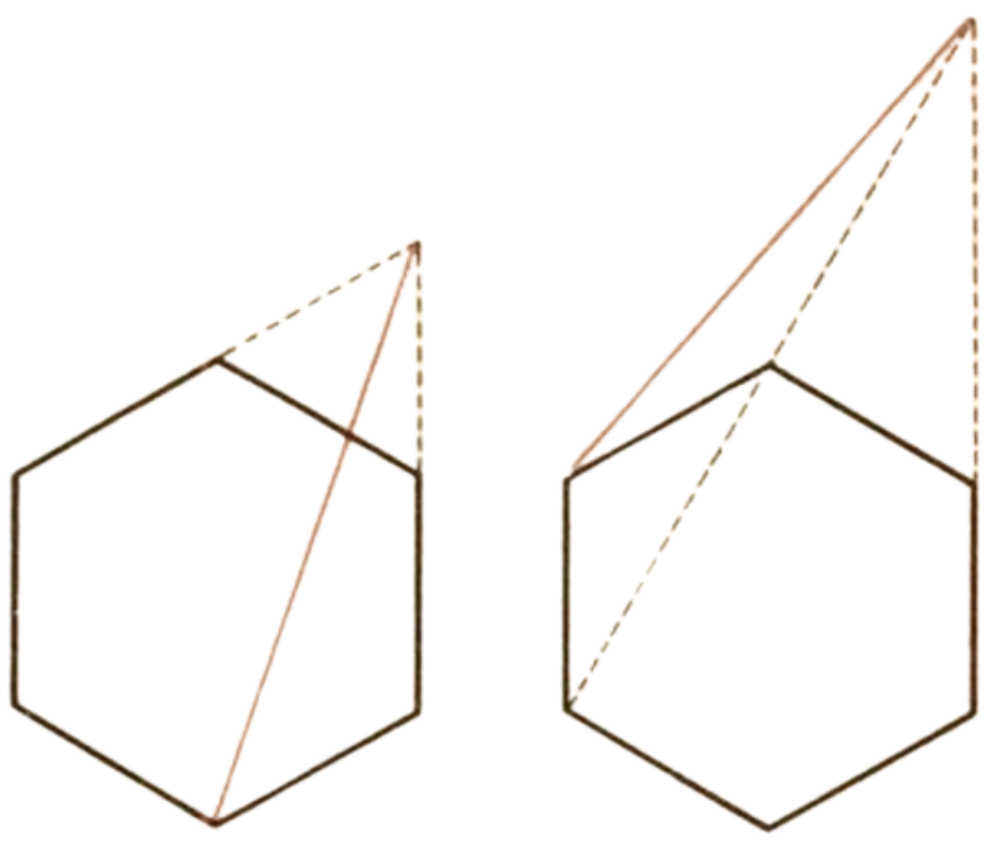
\includegraphics[width=0.92\columnwidth]{hex.png}
        \captionof{figure}{}
    \end{center}
    \noindent\textbf{M172.}
    Докажите, что при любом простом $p$ число $\underbrace{11\dots1}_p$ $\underbrace{22\dots2}_p$ $\underbrace{33\dots3}_p$ \dots $\underbrace{99\dots9}_p$ --- $123456789$ делится на $p$.\par Введём следующие обозначения:
    $123456789 = A$, $\underbrace{11\dots1}_p$ $\underbrace{22\dots2}_p$ $\underbrace{33\dots3}_p$ \dots $\underbrace{99\dots9}_p = B$, $\underbrace{0\dots02}_p$ $\underbrace{0\dots03}_p$ \dots $\underbrace{0\dots08}_p$ $\underbrace{0\dots09}_p = 10^{8p} + 2\cdot10^{7p} + 3\cdot10^{6p} + \dots + 8\cdot10^{p} + 9 = C$, $\underbrace{11\dots1}_p = E$.\par Ясно, что $B = E\cdot C$, $C - A = (10^{8p} - 10^8) + 2(10^{7p} - 10^7) + 3(10^{6p} - 10^6) + \dots +$ $8(10^p-10)$, $10^p - 10  = (9 \cdot E + 1) - 10 = 9(E - 1)$.\par
    \vspace{-4pt}
    \begin{center}
        \begin{tabular}{ |c|c|c|c|c|c| } 
         \hline
         $rad$ & $degree$ & $sin\theta$ & $cos\theta$ & $tan\theta$ & $cot\theta$\\
         \hline
         $0|2\pi$ & $0$ & $0$ & $1$ & $0$ & $\nexists$\\ 
         \hline
         $\pi/6$ & $30^\circ$ & $1/2$ & $\sqrt{3}/2$ & $1/\sqrt{3}$ & $\sqrt{3}$\\ 
         \hline
         $\pi/4$ & $45^\circ$ & $\sqrt{2}/{2}$ & $\sqrt{2}/2$ & $1$ & $1$\\ 
         \hline
         $\pi/3$ & $60^\circ$ & $\sqrt{3}/2$ & $1/2$ & $\sqrt{3}$ & $1/\sqrt{3}$ \\ 
         \hline
         $\pi/2$ & $90^\circ$ & $1$  & $0$ & $\nexists$ & $0$\\
         \hline
        \end{tabular}
    \end{center}
    
    \end{multicols}

